% !TEX program = xelatex
\PassOptionsToPackage{quiet}{fontspec}
\PassOptionsToPackage{dvipsnames}{xcolor}
\documentclass[10pt,aspectratio=169]{beamer}
\usepackage{zju_beamer}
\usepackage{booktabs}
\usepackage{tabularx}
\usepackage{array}
\usepackage{ragged2e}
\usepackage{tikz}
\usetikzlibrary{arrows.meta,positioning,calc}
\graphicspath{{./figures/}}
\zjusectioncolor{blue}

\definecolor{Ink}{RGB}{25,36,52}
\definecolor{Muted}{RGB}{88,99,115}
\definecolor{Accent}{RGB}{0,96,160}
\definecolor{Good}{RGB}{34,135,92}
\definecolor{Warn}{RGB}{196,116,32}
\definecolor{SoftBlue}{RGB}{235,243,252}
\definecolor{SoftGreen}{RGB}{237,248,242}
\definecolor{SoftOrange}{RGB}{255,246,235}

\newcolumntype{Y}{>{\RaggedRight\arraybackslash}X}
\newcommand{\tightitems}{\setlength{\itemsep}{0.24em}}
\newcommand{\smallnote}[1]{\vspace{0.25em}{\scriptsize\textcolor{Muted}{#1}}}
\newcommand{\metric}[3]{%
  \begin{block}{#1}
    \centering
    {\LARGE\bfseries #2}\\[-0.1em]
    {\scriptsize\textcolor{Muted}{#3}}
  \end{block}
}

\title[nlp-cot]{基于大语言模型的思维链推理策略对比研究}
\subtitle{Self-Consistency、Step-Aware Verifier、RAG + CoT、Multi-Agent Debate 与 Harness Engineering}
\author[nlp-cot]{nlp-cot 项目组}
\institute[ZJU]{浙江大学 \quad 自然语言处理课程大作业}
\date{2026 年 6 月}

\begin{document}

\begin{frame}
  \titlepage
\end{frame}

\begin{frame}{汇报结构}
  \tableofcontents
\end{frame}

\section{任务背景}

\begin{frame}{研究任务：在数学应用题上比较 CoT 增强策略}
  \begin{columns}[T,onlytextwidth]
    \begin{column}{0.52\textwidth}
      \begin{block}{选题要求}
        \begin{itemize}
          \tightitems
          \item 面向 AQuA 等推理数据集，分析大语言模型的 Chain-of-Thought 能力。
          \item 复现并比较多路径推理、verifier、检索增强、多 Agent 协作等方法。
          \item 关注准确率、推理成本、工程可复现性与失败案例。
          \item Bonus：用 harness engineering 管理 agentic 推理任务。
        \end{itemize}
      \end{block}
    \end{column}
    \begin{column}{0.44\textwidth}
      \begin{alertblock}{核心问题}
        单条 CoT 容易受采样随机性、答案格式、局部计算错误和自相矛盾影响。
      \end{alertblock}
      \begin{block}{本项目目标}
        在统一实验框架下，把不同策略的收益与成本放在同一把尺子上比较。
      \end{block}
    \end{column}
  \end{columns}
\end{frame}

\begin{frame}{统一实验框架：同一入口、同一数据、同一指标}
  \centering
  \begin{tikzpicture}[
    node distance=0.68cm and 0.82cm,
    box/.style={draw=Accent, rounded corners=2pt, fill=SoftBlue, align=center,
      minimum width=2.55cm, minimum height=0.72cm, font=\small},
    wide/.style={draw=Accent, rounded corners=2pt, fill=blue!10, align=center,
      minimum width=4.2cm, minimum height=0.78cm, font=\small\bfseries},
    arr/.style={-{Latex[length=2mm]}, thick, draw=Accent}
  ]
    \node[wide] (h) {harness.py\\统一实验入口};
    \node[box, below left=of h] (task) {tasks\\AQuATask};
    \node[box, below=of h] (model) {models\\API Wrapper};
    \node[box, below right=of h] (eval) {eval\\metrics};
    \node[wide, below=0.98cm of model] (strategy) {strategies\\Base / SC / Verifier / RAG / Debate / Prefix};
    \node[box, below left=of strategy] (data) {data/AQuA\\test.json};
    \node[box, below=of strategy] (prompt) {prompts\\CoT 模板};
    \node[box, below right=of strategy] (runs) {experiments/runs\\结果 JSON};
    \draw[arr] (h) -- (task);
    \draw[arr] (h) -- (model);
    \draw[arr] (h) -- (eval);
    \draw[arr] (task) -- (strategy);
    \draw[arr] (model) -- (strategy);
    \draw[arr] (strategy) -- (data);
    \draw[arr] (strategy) -- (prompt);
    \draw[arr] (strategy) -- (runs);
    \draw[arr] (eval) -- (runs);
  \end{tikzpicture}
  \smallnote{关键代码：\texttt{harness.py} 负责加载任务、模型、策略并保存实验结果。}
\end{frame}

\section{Self-Consistency}

\begin{frame}{Self-Consistency：从单条推理变成多路径投票}
  \framesubtitle{Self-Consistency Improves Chain of Thought Reasoning in Language Models}
  \begin{columns}[T,onlytextwidth]
    \begin{column}{0.49\textwidth}
      \begin{block}{论文核心思想}
        \begin{itemize}
          \tightitems
          \item 用较高温度采样多条 CoT 推理路径。
          \item 每条路径给出一个最终选项。
          \item 通过聚合答案降低单次采样偶然错误。
        \end{itemize}
      \end{block}
      \begin{block}{原始多数投票}
        \centering
        路径数多的答案获胜：\quad $\arg\max_y \sum_i \mathbb{1}[\hat y_i=y]$
      \end{block}
    \end{column}
    \begin{column}{0.47\textwidth}
      \begin{alertblock}{项目中的改进点}
        多数票不一定代表高质量推理。因此我们负责的 self-consistency 部分改为：
        \[
          \arg\max_y \sum_i q_i \cdot \mathbb{1}[\hat y_i=y]
        \]
        其中 $q_i$ 是第 $i$ 条路径的启发式质量分。
      \end{alertblock}
    \end{column}
  \end{columns}
\end{frame}

\begin{frame}{自适应加权 Self-Consistency：票数之外再看路径质量}
  \begin{columns}[T,onlytextwidth]
    \begin{column}{0.54\textwidth}
      \begin{block}{质量分由什么决定}
        \begin{tabularx}{\linewidth}{lY}
          \toprule
          信号 & 作用 \\
          \midrule
          答案清晰 & 是否严格输出 \texttt{Answer: X} \\
          推理步骤 & 是否有显式 step 或分段推理 \\
          数学痕迹 & 是否包含数字、运算符、等式等计算信号 \\
          输出长度 & 过短扣分，过长轻微扣分 \\
          自相矛盾 & 多处答案不一致时扣分 \\
          \bottomrule
        \end{tabularx}
      \end{block}
    \end{column}
    \begin{column}{0.42\textwidth}
      \begin{block}{一个直观例子}
        \small
        \begin{tabular}{lcc}
          \toprule
          答案 & 路径数 & 加权票 \\
          \midrule
          A & 2 & $1.8 + 1.7 = 3.5$ \\
          B & 3 & $0.8 + 0.7 + 0.6 = 2.1$ \\
          \bottomrule
        \end{tabular}
        \smallskip

        旧算法选 B，因为 B 有 3 票；新算法选 A，因为 A 的两条推理更清晰、更完整。
      \end{block}
      \begin{alertblock}{边界}
        该方法只使用本路径文本的局部信号，不调用 verifier、不检索外部知识，也不引入多 Agent。
      \end{alertblock}
    \end{column}
  \end{columns}
\end{frame}

\begin{frame}[fragile]{结合真实代码：self\_consistency.py 的执行流程}
  \begin{columns}[T,onlytextwidth]
    \begin{column}{0.49\textwidth}
      \begin{block}{关键函数}
        \begin{itemize}
          \tightitems
          \item \texttt{\_path\_quality}: 计算每条路径的启发式质量分。
          \item \texttt{\_aggregate\_votes}: 按权重聚合，并用原始票数、最佳路径质量、出现顺序打破平票。
          \item \texttt{\_can\_stop\_early}: 当领先答案无法被剩余路径追上时提前停止。
          \item \texttt{run}: 生成路径、抽取答案、重试空答案、聚合最终预测。
        \end{itemize}
      \end{block}
    \end{column}
    \begin{column}{0.47\textwidth}
      \begin{block}{伪代码}
        \scriptsize
\begin{verbatim}
for i in range(n_paths):
    raw = model.generate(prompt, temperature)
    pred = task.extract_answer(raw)
    if retry_on_empty and not pred:
        raw = model.generate(prompt, low_temp)
    weight = _path_quality(raw, pred)
    save(pred, weight)
    if _can_stop_early(...):
        break

final = _aggregate_votes(predictions, weights)
\end{verbatim}
      \end{block}
      \smallnote{低温重试让模型输出更稳定，主要用于补救没有 \texttt{Answer: X} 的样本。}
    \end{column}
  \end{columns}
\end{frame}

\section{Step-Aware Verifier}

\begin{frame}{Step-Aware Verifier：从“看最终答案”到“看每一步”}
  \framesubtitle{Making Large Language Models Better Reasoners with Step-Aware Verifier}
  \begin{columns}[T,onlytextwidth]
    \begin{column}{0.49\textwidth}
      \begin{block}{论文思想}
        \begin{itemize}
          \tightitems
          \item 把推理过程拆成 step。
          \item 对每一步进行正确性或可信度评估。
          \item 用 verifier 选择更可靠的推理路径。
        \end{itemize}
      \end{block}
    \end{column}
    \begin{column}{0.47\textwidth}
      \begin{block}{项目实现}
        \begin{itemize}
          \tightitems
          \item 策略入口：\texttt{strategies/step\_verifier.py}。
          \item verifier 模型封装：\texttt{models/deberta\_verifier.py}。
          \item 结果保存 step 级评分，用于选择最终答案。
        \end{itemize}
      \end{block}
      \begin{alertblock}{实验观察}
        AQuA 前 100 条达到 94\%，但平均输出 token 与耗时明显高于 base/self-consistency。
      \end{alertblock}
    \end{column}
  \end{columns}
\end{frame}

\section{RAG + CoT}

\begin{frame}{RAG + CoT：用外部知识补足纯参数记忆}
  \framesubtitle{Interleaving Retrieval with Chain-of-Thought Reasoning for Knowledge-Intensive Multi-Step Questions}
  \begin{columns}[T,onlytextwidth]
    \begin{column}{0.49\textwidth}
      \begin{block}{论文思想}
        \begin{itemize}
          \tightitems
          \item 在推理过程中穿插检索。
          \item 把 retrieved evidence 与 CoT 推理交替组织。
          \item 适合知识密集型、多跳问答。
        \end{itemize}
      \end{block}
    \end{column}
    \begin{column}{0.47\textwidth}
      \begin{block}{项目实现与局限}
        \begin{itemize}
          \tightitems
          \item 策略入口：\texttt{strategies/rag\_cot.py}。
          \item 对 AQuA 这类数学题，检索信息不总是关键瓶颈。
          \item 输入 token 上升明显；收益依赖检索质量与任务类型。
        \end{itemize}
      \end{block}
      \begin{alertblock}{实验观察}
        100 样本准确率 92\%，高于 base 但低于 self-consistency 与 verifier。
      \end{alertblock}
    \end{column}
  \end{columns}
\end{frame}

\section{Multi-Agent Debate}

\begin{frame}{Multi-Agent Debate：让多个角色协作、反驳与裁决}
  \framesubtitle{Improving Factuality and Reasoning in Language Models through Multiagent Debate}
  \centering
  \begin{tikzpicture}[
    node distance=0.58cm and 0.72cm,
    role/.style={draw=Accent, rounded corners=2pt, fill=SoftBlue, align=center,
      minimum width=2.65cm, minimum height=0.75cm, font=\small},
    judge/.style={draw=Good, rounded corners=2pt, fill=SoftGreen, align=center,
      minimum width=3.25cm, minimum height=0.82cm, font=\small\bfseries},
    arr/.style={-{Latex[length=2mm]}, thick, draw=Accent}
  ]
    \node[role] (a1) {Agent 1\\独立推理};
    \node[role, right=of a1] (a2) {Agent 2\\独立推理};
    \node[role, right=of a2] (a3) {Agent 3\\独立推理};
    \node[role, below=0.9cm of a2] (debate) {讨论 / 反思\\指出错误与证据};
    \node[judge, below=0.88cm of debate] (vote) {裁决或汇总\\输出最终答案};
    \draw[arr] (a1) -- (debate);
    \draw[arr] (a2) -- (debate);
    \draw[arr] (a3) -- (debate);
    \draw[arr] (debate) -- (vote);
  \end{tikzpicture}

  \vspace{0.4em}
  \begin{columns}[T,onlytextwidth]
    \begin{column}{0.49\textwidth}
      \begin{block}{项目实现}
        \small \texttt{strategies/multi\_agent\_debate.py} 中模拟多角色生成、互评与最终汇总。
      \end{block}
    \end{column}
    \begin{column}{0.47\textwidth}
      \begin{alertblock}{实验观察}
        100 样本准确率 95\%，但真实 API 成本高于保存结果中展示的最终摘要 token。
      \end{alertblock}
    \end{column}
  \end{columns}
\end{frame}

\section{Bonus: Harness Engineering}

\begin{frame}{Bonus：用 Harness Engineering 管理 agentic 任务}
  \framesubtitle{参考：\url{https://github.com/walkinglabs/learn-harness-engineering}}
  \begin{columns}[T,onlytextwidth]
    \begin{column}{0.54\textwidth}
      \begin{block}{为什么需要 harness}
        \begin{itemize}
          \tightitems
          \item 多策略、多参数、多 API 后端很容易变成不可复现实验。
          \item Harness 把任务、模型、策略、指标、结果保存拆成稳定接口。
          \item 便于替换个人负责的 \texttt{strategies/*.py}，不影响其他同学模块。
        \end{itemize}
      \end{block}
    \end{column}
    \begin{column}{0.42\textwidth}
      \begin{block}{子系统覆盖}
        \small
        \begin{tabular}{lcccc}
          \toprule
          策略 & 指令 & 环境 & 状态 & 反馈 \\
          \midrule
          Base & 是 & 是 & 否 & 否 \\
          SC & 是 & 是 & 是 & 否 \\
          Verifier & 是 & 是 & 是 & 是 \\
          RAG & 是 & 是 & 是 & 部分 \\
          Debate & 是 & 是 & 是 & 是 \\
          \bottomrule
        \end{tabular}
      \end{block}
    \end{column}
  \end{columns}
\end{frame}

\section{实验结果}

\begin{frame}{实验设置：AQuA test 前 100 条，统一 API 调用}
  \begin{columns}[T,onlytextwidth]
    \begin{column}{0.33\textwidth}
      \metric{数据集}{AQuA}{test split 前 100 条}
    \end{column}
    \begin{column}{0.33\textwidth}
      \metric{模型接口}{API}{DMXAPI / DeepSeek 兼容格式}
    \end{column}
    \begin{column}{0.33\textwidth}
      \metric{评估指标}{Accuracy}{同时记录 token、步数、耗时}
    \end{column}
  \end{columns}

  \vspace{0.6em}
  \begin{block}{运行方式示例}
    \small
    \texttt{python harness.py --strategy self\_consistency --dataset aqua --n\_samples 100 --n\_paths 7}
  \end{block}
\end{frame}

\begin{frame}{100 样本准确率：多路径与协作方法整体领先}
  \begin{columns}[T,onlytextwidth]
    \begin{column}{0.58\textwidth}
      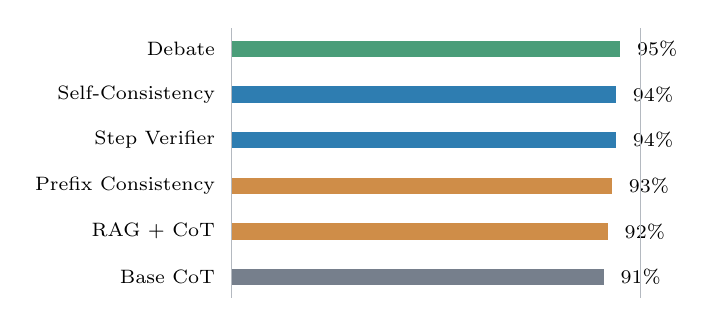
\begin{tikzpicture}[x=0.052cm,y=0.58cm]
        \scriptsize
        \foreach \name/\acc/\y/\col in {
          Debate/95/0/Good,
          Self-Consistency/94/1/Accent,
          Step Verifier/94/2/Accent,
          Prefix Consistency/93/3/Warn,
          RAG + CoT/92/4/Warn,
          Base CoT/91/5/Muted}
        {
          \node[anchor=east] at (0,-\y) {\name};
          \fill[\col!82] (2,-\y-0.18) rectangle (2+\acc,-\y+0.18);
          \node[anchor=west] at (2+\acc+2.2,-\y) {\acc\%};
        }
        \draw[Muted!45] (2,0.45) -- (2,-5.45);
        \draw[Muted!45] (102,0.45) -- (102,-5.45);
      \end{tikzpicture}
    \end{column}
    \begin{column}{0.38\textwidth}
      \begin{block}{结论}
        \begin{itemize}
          \tightitems
          \item Base CoT 已有 91\% 基线。
          \item Self-Consistency 提升到 94\%，收益稳定且工程侵入小。
          \item Debate 最高为 95\%，但成本与调度复杂度更高。
        \end{itemize}
      \end{block}
    \end{column}
  \end{columns}
\end{frame}

\begin{frame}{效率对比：准确率提升背后有不同成本}
  \small
  \begin{tabularx}{\linewidth}{lrrrrY}
    \toprule
    策略 & 样本 & 正确 & 准确率 & 平均输出 & 观察 \\
    \midrule
    Base CoT & 100 & 91 & 91\% & 187.64 & 单路径，成本最低。 \\
    Self-Consistency & 100 & 94 & 94\% & 238.56 & 多路径采样，准确率稳定提升。 \\
    Step Verifier & 100 & 94 & 94\% & 563.74 & step 级评估更细，但输出成本最高。 \\
    RAG + CoT & 100 & 92 & 92\% & 197.90 & 输入 token 增加，受检索质量影响。 \\
    Multi-Agent Debate & 100 & 95 & 95\% & 72.18 & 结果文件只保存摘要，实际调用成本更高。 \\
    \bottomrule
  \end{tabularx}
  \smallnote{单位为实验 JSON 记录的平均 output tokens；Debate 的记录低估了真实中间讨论成本。}
\end{frame}

\begin{frame}{50 到 100 样本稳定性：Self-Consistency 最稳}
  \begin{columns}[T,onlytextwidth]
    \begin{column}{0.52\textwidth}
      \small
      \begin{tabular}{lcc}
        \toprule
        策略 & 前 50 条 & 前 100 条 \\
        \midrule
        Multi-Agent Debate & 94\% & 95\% \\
        Self-Consistency & 94\% & 94\% \\
        Step Verifier & 92\% & 94\% \\
        Prefix Consistency & 94\% & 93\% \\
        RAG + CoT & 78\% & 92\% \\
        Base CoT & 92\% & 91\% \\
        \bottomrule
      \end{tabular}
    \end{column}
    \begin{column}{0.44\textwidth}
      \begin{block}{分析}
        \scriptsize
        \begin{itemize}
          \tightitems
          \item Self-Consistency 在 50/100 样本上均为 94\%，波动最小。
          \item RAG 前 50 条偏低，对样本分布和检索质量更敏感。
          \item Debate 准确率最高，但更适合作为高成本上限方案。
        \end{itemize}
      \end{block}
    \end{column}
  \end{columns}
\end{frame}

\section{总结}

\begin{frame}{方法对比总结：不同策略解决不同失败模式}
  \small
  \begin{tabularx}{\linewidth}{lYYY}
    \toprule
    方法 & 主要解决的问题 & 优势 & 局限 \\
    \midrule
    Self-Consistency & 单路径随机错误 & 简单、低风险、可直接替换策略文件 & 多次采样增加调用成本 \\
    Step Verifier & 中间步骤错误 & 可解释性强，能定位 step 级问题 & verifier 依赖与耗时较高 \\
    RAG + CoT & 外部知识不足 & 对知识密集题更有潜力 & 数学题收益受检索质量限制 \\
    Debate & 单模型视角偏差 & 多角色互相纠错，准确率最高 & 调度复杂、成本最高 \\
    Harness & 实验不可复现 & 统一接口、结果留痕、便于协作 & 需要规范每个策略的输入输出 \\
    \bottomrule
  \end{tabularx}
\end{frame}

\begin{frame}{结论：本项目的核心贡献}
  \begin{columns}[T,onlytextwidth]
    \begin{column}{0.49\textwidth}
      \begin{block}{算法贡献}
        \begin{itemize}
          \tightitems
          \item 将普通 self-consistency 从“多数投票”改为“自适应加权投票”。
          \item 加入答案有效性检查、空答案低温重试、早停剪枝和平票质量打破。
          \item 不占用 verifier、RAG、debate 的方法边界，只用本路径文本启发式信号。
        \end{itemize}
      \end{block}
    \end{column}
    \begin{column}{0.47\textwidth}
      \begin{block}{工程贡献}
        \begin{itemize}
          \tightitems
          \item 统一策略接口，方便各成员替换 \texttt{strategies} 下自己的方法。
          \item 实验结果自动写入 \texttt{experiments/runs}，便于复查与报告。
          \item 支持 API key / base url / model 参数化，避免硬编码密钥。
        \end{itemize}
      \end{block}
    \end{column}
  \end{columns}
\end{frame}

\begin{frame}{代码与参考}
  \begin{block}{核心代码路径}
    \small
    \begin{tabularx}{\linewidth}{lY}
      \toprule
      路径 & 作用 \\
      \midrule
      \texttt{harness.py} & 统一实验入口与结果保存。 \\
      \texttt{strategies/self\_consistency.py} & 自适应加权 self-consistency。 \\
      \texttt{strategies/step\_verifier.py} & Step-aware verifier 策略。 \\
      \texttt{strategies/rag\_cot.py} & 检索增强 CoT。 \\
      \texttt{strategies/multi\_agent\_debate.py} & 多 Agent debate。 \\
      \texttt{experiments/runs/*.json} & 实验结果与逐样本输出。 \\
      \bottomrule
    \end{tabularx}
  \end{block}
  \begin{block}{参考论文}
    \scriptsize
    Self-Consistency Improves Chain of Thought Reasoning in Language Models;
    Making Large Language Models Better Reasoners with Step-Aware Verifier;
    Interleaving Retrieval with Chain-of-Thought Reasoning for Knowledge-Intensive Multi-Step Questions;
    Improving Factuality and Reasoning in Language Models through Multiagent Debate.
  \end{block}
\end{frame}

\begin{frame}
  \centering
  \vspace{2.2cm}
  {\Huge 谢谢！}\\[0.8em]
  {\large 欢迎提问}
\end{frame}

\end{document}
